\subsection{Recorded retained utility lift}\label{app:retained-utility-lift}

\Cref{fig:fw-retained-utility-lift} subtracts one fixed recorded incumbent
from each post-decision retained score. The prefix uses one logged evaluation
identity and includes all completed decisions through its capture cutoff.
These adaptive observations retain the source-binding and evaluation
limits in \cref{sec:method-status}.

\begin{figure}[htbp]
  \centering
  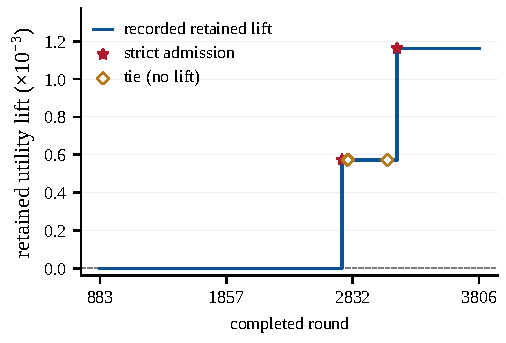
\includegraphics[width=\linewidth]{figures/fig_fw_retained_utility_lift.pdf}
  \caption{\textbf{Retained utility rises in two steps above the round-882 incumbent.}
  All \num{2924} completed records in rounds 883--3806, captured at 17:33 UTC
  on 2 November 2026. Each step is
  $\Delta u_r=u_{\mathrm{best},r}-u_{\mathrm{best},882}$, using the same
  recorded round-882 incumbent throughout. Vertical tick values denote
  $10^{-3}$ logged utility units. Stars mark two accepted strict gains;
  hollow diamonds mark two accepted ties, which add no lift. The other
  \num{2920} decisions are rejections. Classification uses unrounded logged
  values. Repeated development reuse prevents treating this curve as an
  independent learning or proposal-quality result. Scope: \cref{sec:method-status}.}
  \label{fig:fw-retained-utility-lift}
\end{figure}
